\documentclass[conference]{IEEEtran}
\IEEEoverridecommandlockouts
% The preceding line is only needed to identify funding in the first footnote. If that is unneeded, please comment it out.
\usepackage{cite}
\usepackage{amsmath,amssymb,amsfonts}
\usepackage{algorithmic}
\usepackage{graphicx}
\usepackage{textcomp}
\usepackage{xcolor}
\usepackage{listings}

\definecolor{codegreen}{rgb}{0,0.6,0}
\definecolor{codeblue}{rgb}{0,0,0.6}
\definecolor{codegray}{rgb}{0.5,0.5,0.5}
\definecolor{codepurple}{rgb}{0.58,0,0.82}
\definecolor{backcolour}{rgb}{0.95,0.95,0.92}

\lstdefinestyle{mystyle}{
    backgroundcolor=\color{backcolour},   
    commentstyle=\color{codeblue},
    keywordstyle=\color{codegreen},
    numberstyle=\tiny\color{codegray},
    stringstyle=\color{codepurple},
    basicstyle=\ttfamily\footnotesize,
    breakatwhitespace=false,         
    breaklines=true,                 
    captionpos=b,                    
    keepspaces=true,                 
    showspaces=false,                
    showstringspaces=false,
    showtabs=false,                  
    tabsize=2
}

\lstset{style=mystyle}

\def\BibTeX{{\rm B\kern-.05em{\sc i\kern-.025em b}\kern-.08em
    T\kern-.1667em\lower.7ex\hbox{E}\kern-.125emX}}
\begin{document}

\title{\LARGE \textbf{ Analysis of emotions towards programming languages\\ throughout the 2010s}}

\makeatletter
\newcommand{\linebreakand}{%
  \end{@IEEEauthorhalign}
  \hfill\mbox{}\par
  \mbox{}\hfill\begin{@IEEEauthorhalign}
}
\makeatother

\author{\IEEEauthorblockN{Ishan Chopra}
\IEEEauthorblockA{\textit{Department of Computer Science} \\
\textit{University of Manitoba}\\
Winnipeg, MB, CA \\
choprai@myumanitoba.ca}
\and
\IEEEauthorblockN{Chad Hillary}
\IEEEauthorblockA{\textit{Department of Computer Science} \\
\textit{University of Manitoba}\\
Winnipeg, MB, CA \\
hillaryc@myumanitoba.ca}
\and
\IEEEauthorblockN{Evan Nagasaka}
\IEEEauthorblockA{\textit{Department of Computer Science} \\
\textit{University of Manitoba}\\
Winnipeg, MB, CA \\
umnagasa@myumanitoba.ca}
\linebreakand
\IEEEauthorblockN{Ovietobore Oghre}
\IEEEauthorblockA{\textit{Department of Computer Science} \\
\textit{University of Manitoba}\\
Winnipeg, MB, CA \\
oghreo@myumanitoba.ca}
\and
\IEEEauthorblockN{Earl Placido}
\IEEEauthorblockA{\textit{Department of Computer Science} \\
\textit{University of Manitoba}\\
Winnipeg, MB, CA \\
placidej@myumanitoba.ca}
}

\maketitle

\begin{abstract}
Stack Overflow is widely used by software developers all around the world and is one of the most commonly used platforms to get help with programming-related issues. But since it uses a Question-Answer model, the quality of discussion can often depend on the sentiment conveyed through questions, answers, and comments. Trends in technology keep shifting and popular technologies can easily become forgotten and obsolete. As such, developers' feelings towards different programming languages and tools continue to change as new programming languages and tools emerge. In this project, we applied sentimental analysis techniques to Stack Overflow data to find interesting patterns about developers' feelings towards some languages over time. The nature of Software Engineering texts causes normal Sentimental Analysis tools to have questionable results. So we used Senti4SD, which is a classifier trained on Software Engineering data.
\end{abstract}

\begin{IEEEkeywords}
Sentiment Analysis, Stack Overflow, Empirical Software Engineering, Natural Language Processing, Visualization, Qualitative Analysis
\end{IEEEkeywords}

\section{Introduction}
As technology becomes more ubiquitous with everyday life, developers and engineers have continued to innovate and develop new technological tools and programming languages (these terms are used interchangeably from here on out) to solve newer problems or to bring a new perspective into the process of developing new software. With newer tools emerging, developers' feelings towards existing and novel tools changes over time. Our aim is to find interesting patterns related to that change in developer feelings. \\

Stack Overflow is used by most developers, for work and/or for personal projects. Questions and answers are posted by newcomers and experienced professionals, and everyone in between. Its ubiquity, active community, and open source data makes for a representative data source with enough entries to allow meaningful analysis about developer feelings about different tools over time. So, we used data from Stack Overflow as the base for our research. Stack Overflow data also contains dates and tags. This makes collection of language-specific posts easy and also helps with temporal analysis that we aim to do.

\subsection{Motivation}
Emotional awareness plays a critical role in collaborative work. Software development is highly collaborative and depends on a lot of collaborations tools like email, forums, code repositories, and issue tracking tools\cite{b1}. Previous research shows that emotion in the workplace affects collaboration and productivity of employees\cite{b2}. \\

Discussions on StackOverflow aren't neutral. Previous research suggests that a sizable amount of texts are positive or negative\cite{b3, b4, b5}. There is also evidence that Stack Overflow can be perceived as a hostile environment, particularly for newcomers\cite{b6}. We wanted to go through data over the years and to find how developers' emotions towards different languages has changed over the years to answer the following questions:
 \subsubsection{Trends}Are there any interesting trends about developers' changing emotions towards languages?
 \subsubsection{Comparisons}How do newer languages compare to the established ones and obsolete ones?
 \subsubsection{Compiled vs Interpreted}How do emotions towards compiled languages differ from emotions towards interpreted languages over time?
 \subsubsection{Type}How do questions compare to answers?\\

So we aim to use NLP techniques and the data we have gathered to answer these questions.

\subsection{Our Contribution}
We researched NLP tools and techniques that would help use with this problem. We collected data for multiple languages from Stack Overflow and applied Sentimental analysis techniques along with temporal analysis to answer interesting questions about developers' emotions towards different languages over time and how these might be connected to other attributes of the language like age, maturity, and runtime nature.\\

\section{Background}

\subsection{Natural Language Processing}
Natural Language Processing is the extraction of meaning from human language using a computer\cite{b7, b8}. Some of the applications of NLP include translation, text retrieval, dialogue systems, information summarization, and categorization\cite{b7}. While NLP began as an intersection of AI and Linguistics in the 1950s, it has evolved to use statistical methods and borrows from many diverse fields including Machine Learning, Data Science, and AI \cite{b8}. \\

While earlier methods used  rules and determinism, newer techniques use probabilities and statistics in the form of machine learning \cite{b8}. NLP is a challenging problem due to the complex nature of human language and this means that rule-based systems were limited in what they could achieve. Our focus is on the Sentiment Analysis, which is a subfield of NLP. \\

\subsection{Sentiment Analysis}
Sentiment Analysis deals with the computational treatment of opinion, sentiment, and subjectivity in text. Sentiment Analysis techniques aim to identify polarity in a sentence or document. More formally, it is the discovery of sentiment expressed by an opinion holder towards some entities such as products, services, people, companies, issues, or events. Document-level sentiment analysis treats the whole document as an entity, while sentence-level classification assigns a sentiment to each sentence. There are many applications of Sentiment Analysis like product review understanding, recommendations, QnA sites, social media, company reputation and opinion, politics, and marketing. \cite{b10, b13, b19}\\

Some of the common methods of Sentiment Analysis include machine learning methods and lexical-based approaches. Lexical-based methods use predefined lists of words and n-grams in which each word is associated with different sentiments. As a result, the methods vary based on the context they are applied to and aren't directly usable in a different context. Some examples of lexical based methods include Linguistic Inquiry and Word Count (LWIC), SO-CAL, and VADER.\cite{b11, b13}\\

Machine learning approaches to Sentiment Analysis can be divided into supervised or unsupervised methods. The former has the advantage that models can be trained or adapted for specific purposes and contexts (like Software Engineering texts) using properly labelled data. The disadvantage is that it is hard to apply results to other domains. Some of the commonly considered features include negations, n-grams, word frequencies, part of speech tagging, opinion words and phrases, and presence of words. Classifiers using SVMs and Naive Bayes classifiers are effective for sentence-level Sentiment Analysis.\cite{b11, b13, b14}\\

Some of the newer sentiment analyzers combine the lexical-based methods and machine learning methods. Examples include SentiWordNet\cite{b15}, SentiStrength\cite{b16}, and Standford recursive deep model\cite{b17}.\\

An in-depth study on 24 published sentiment analyzers found that different analysers have different performance depending on the dataset used. It also shows that these analyzers may not agree with each other. This means very different results based on the analyzer used. This means that it is important to choose to right analyzer for the domain and application. This is also the biggest threat to validity for our study.\\

\begin{figure}[htbp]
\centerline{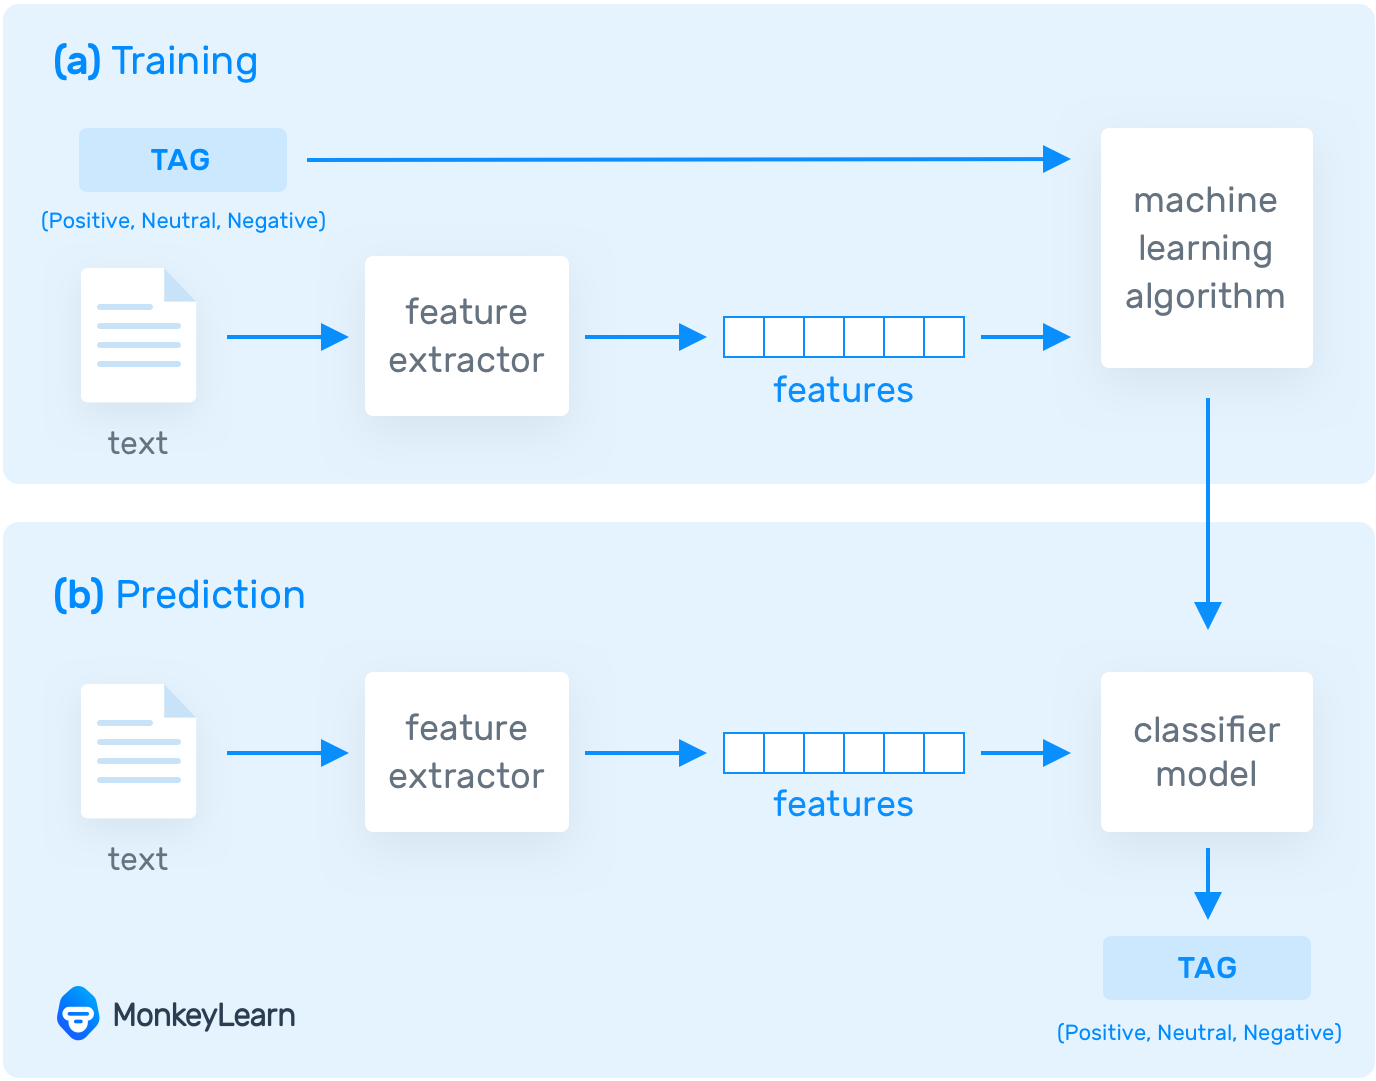
\includegraphics[width=0.49\textwidth]{how-does-sentiment-analysis-work.png}}
\caption{An illustration of how ML-based Supervised Sentiment Analyzers work\cite{b32}}
\label{fig}
\end{figure}

\section{Related Work}
Prior work on sentimental analysis in development environment have been largely divided into two categories, namely; evaluation of analyzers and classifier for sentimental analysis and study on effects of emotion in developer environments\\


\subsection{Evaluation of Sentiment Analysis Tools}
Many of the empirical Software Engineering studies rely on off the shelf analyzers that are not trained on Software Engineering domain-specific texts. The research community questions the validity of these results\cite{b21}. To overcome this limitations, a few analyzers have been created for the Software Engineering domain.\\ 

The publicly available Sentiment Analysis tools that we considered were SentiStrength, Senti4SD, SentiStrengthSE, and SentiCR\cite{b16, b18, b19, b20}. We picked these over some of the newer models like BERT\cite{b22} due to the shorter nature of the project and the fact that these have been available publicly and have been tested extensively in the Software Engineering (SE) domain. Ultimately, we went with Senti4SD due to it's accuracy on Stack Overflow Data, public availability and the thorough research done on it (maturity).\\

\subsubsection{SentiStrength}
SentiStrength is a well performing lexical-based classifier that deals with short texts. The core of the algorithm is a lexicon where words receive a score representing their apriori (out-of-context) polarity. The scores range from 2 to 5 (or -2 to -5 for negative comments). \\

Given the assumption that sentences can convey multiple emotions, SentiStrength considers both postive and negative sentiment scores for each sentence. For negations, it inverts the polarity scores. It considers repeated punctuation, exclamation, and booster words (like "very", "extremely", etc.) to increase or decrease the polarity. When dealing with documents, SentiStrength considers maximum values from each sentence, and assigns a score based on a 1-5 scale (and -1 to -5 scale for negative emotions). It can also report a trinary document score (-1, 0, +1). This is one of the most widely used Sentiment Analysis tools.\cite{b16, b21}\\

\subsubsection{SentiStrengthSE}
SentiStrengthSE is a SE-specific sentiment analysis tool built using the SentiStrength API\cite{b20}. Published in 2017, it builds on SentiStrength and uses a manually adjusted version of the SentiStrength lexicon along with ad-hoc heuristics to correct misclassifications. The polarity scores were manually adjusted to reflect the neutral polarity of terms that are perceived as negative outside of the SE domain. The authors of SentiStrengthSE used a "gold standard" dataset\cite{b23} found that it significantly outperforms SentiStrength on SE related texts\cite{b20}.\\

Some of the difficulties that they faced and addressed are also faced by other researchers, both in the SE-specific domain and outside it. These include
\begin{itemize}
    \item Domain-specific meanings of words
    \item Context-sensitive variations in meanings of words
    \item Difficulty with negations
    \item Missing words in the dictionary
    \item Sentimental words in interrogative sentences (questions)
    \item Difficulty detecting irony and sarcasm
    \item Subtle expressions of sentiment\\
\end{itemize}

\subsubsection{SentiCR}
SentiCR is a supervised learning sentiment analyzer, trained specifically for Code review comments using data from Gerritt. It uses a feature vector generated by computing the Term Frequency - Inverse Document Frequency (TF-IDF) for words extracted from input text. As with SentiStrengthSE, it also has a preprocessing step to deal with some of the challenges mentioned and to normalize text. It performs synthetic minority over-sampling technique (SMOTE) to address class imbalance in training data by improving the ratio of negative to non-negative comments in the training sequence. The authors found that the Gradient Boosting Tree performs the best out of the Supervised learning approaches they used\cite{19} (like Adaptive Boosting, Naive Bayes, SVM with Schotastic Gradient Descent, etc.).\\

\subsubsection{Senti4SD}
Senti4SD is a sentiment analyzer created in 2017 for software development related texts. The authors came up with a manually annotated gold standard dataset built based on more than 4000 Stack Overflow questions, answers, and comments. This complements the gold standard dataset that the SentiStrengthSE authors used. It considers various features including 19 Lexicon-based features, 76,346 Keyword-based features, and 4 Semantic features\cite{b18}. For the Semantic features, Senti4SD contains a Distributed Semantic Model (DSM) trained with 20 million preprocessed documents from Stack Overflow. In a DSM, linguistic items (like words, sentences, and documents) are represented as vectors is a high dimensional space. Senti4SD is trained with SVMs because SVMs are able to learn and generalize even in high dimensional feature space like the one Senti4SD has.\\

Compared to SentiStrength, Senti4SD reduces misclassifications of neutral and positive posts as negative \cite{b21}. Overall, Senti4SD outperforms or is close in performance to SentiStrength, SentiCR, and SentiStrengthSE for different SE-specific data\cite{b21, b26}. But Senti4SD is better than SentiStrength, SentiCR, and SentiStrengthSE for Stack Overflow data. This is the primary reason we picked Senti4SD for our purposes. It is noted that different sentiment analyzers might give different results, but the conclusions can be consistent at a coarse level of granularity \cite{b26}.\\

\subsubsection{BERT*}
Bidirectional Encoder Representations from Transformers (BERT) is a relatively new model that performs really well at sentiment analysis on general texts\cite{b27}. While it has the potential to be much better than existing techniques for SE-specific texts, it is not at that stage yet. BERT has been applied to SE-specific data with some success\cite{b22}, but empirical research shows that it doesn't outperform Senti4SD by a meaningful amount \cite{b26}. This would make for an interesting comparison in the future, but under the time constraints, we went with Senti4SD for our task due to its maturity and good performance on Stack Overflow data. \\

\begin{figure*}[tbp]
\centering
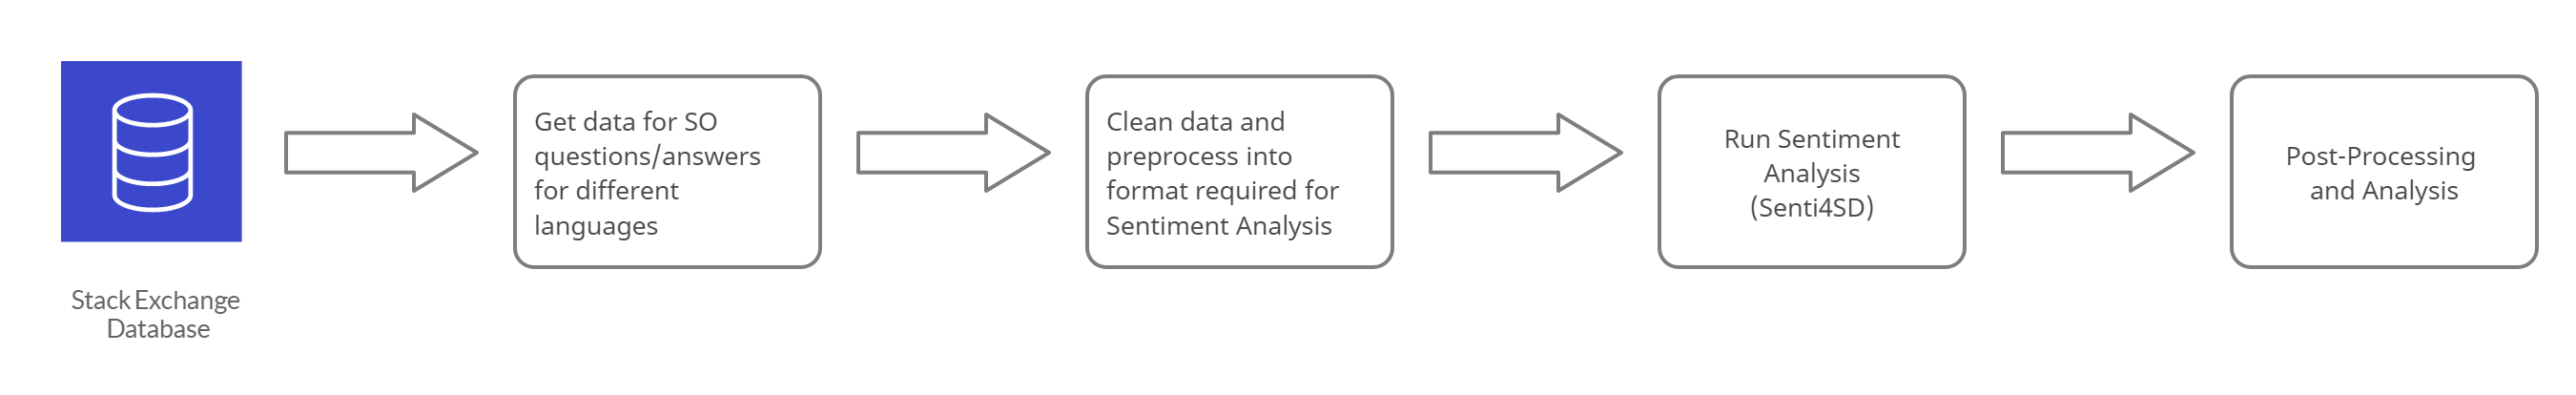
\includegraphics[width=\textwidth]{4710_method_summary.png}
\caption{Overview of how we approached the problem}
\label{fig}
\end{figure*}

\subsection{Emotions in Software Engineering and Stack Overflow}
While there has been plenty of research into performing Sentiment Analysis on SE-related data, there is not much research into the results obtained from these Sentiment Analysis techniques. Novielli et al\cite{b33} used information from stack overflow data to argue that the emotional style of a technical question affects the probability of said question getting an appropriate answer.  Ling and Larsen\cite{b11} have also applied the Senti4SD model to Stack Overflow Data for some popular languages, however, in that paper, they used only data from 2017 and did not consider any changes in the sentiments over a more extensive time period. From our research, most of the work done using stack overflow data has been more qualitative that quantitative. For example, Novielle et al \cite{b34} presented a qualitative overview of the different types of positive and negative emotions in questions and answers. But to the best of our knowledge no one has used Sentiment Analysis on Stack Overflow data to find interesting changes and trends over time. Software development is always in a state of flux, so we believe there are some interesting patterns than can be uncovered by our type of analysis.\\

\section{Our Method}
 
\subsection{Overview}
We wanted to get a good subset of programming languages for our analysis, but not so many that it would become very time consuming. We planned to use the StackExchange data dump for Stack Overflow, but it proved to be a bit too expensive computationally and for storage. So, our current approach involved randomly sampling data from Stack Overflow for different languages using the Stack Exchange API. While the API had a cap of 50,000 entries per query, this was sufficient for our purposes. We cleaned and preprocessed the data into a format that the Senti4SD classifier requires and then ran the classifier for different programming languages and different time periods. A summary is provided in Figure 2.\\

\begin{table}[htbp]
\caption{Programming Languages selected}
\begin{center}
\begin{tabular}{|c|c|c|}
\hline
\textbf{Language}&\textbf{Compiled/Interpreted}& \textbf{New/Old}\\
\hline
C&Compiled&Old\\
\hline
C++&Compiled&Old\\
\hline
Java&Compiled&Old\\
\hline
Rust&Compiled&New\\
\hline
Ruby/Rails&Compiled&Old\\
\hline
Python&Interpreted&Old\\
\hline
Perl&Interpreted&Old\\
\hline
JavaScript&Interpreted&Old\\
\hline
\end{tabular}
\label{tab1}
\end{center}
\end{table}

Information about the languages we picked is in Table I. As seen in the Stack Overflow 2020 survey\cite{b29}, these are among the most popular languages and people have very positive attitudes towards some of these languages. This information is summarized in Table II and III. In Table III, the languages with less than 50\% in their row are the ones that are theoretically not liked by users. Perl, at 29.4\% ranks even below Assembly in the Stack Overflow survey's likability section.\\

\begin{table}[htbp]
\caption{Popular Programming Languages on Stack Overflow}
\begin{center}
\begin{tabular}{|c|c|}
\hline
\textbf{Rank}&\textbf{Language}\\
\hline
1&JavaScript\\
\hline
4&Python\\
\hline
5&Java\\
\hline
10&C++\\
\hline
11&C\\
\hline
14&Ruby\\
\hline
19&Rust\\
\hline
23&Perl\\
\hline
\end{tabular}
\label{tab1}
\end{center}
\end{table}

\begin{table}[htbp]
\caption{Most liked/dreaded languages on Stack Overflow}
\begin{center}
\begin{tabular}{|c|c|}
\hline
\textbf{Language}&\textbf{\% of Devs who use it and will continue to use it}\\
\hline
Rust&86.1\%\\
\hline
Python&66.7\%\\
\hline
JavaScript&58.3\%\\
\hline
Java&44.1\%\\
\hline
C++&43.4\%\\
\hline
Ruby&42.9\%\\
\hline
C&33.1\%\\
\hline
Perl&29.4\%\\
\hline
\end{tabular}
\label{tab1}
\end{center}
\end{table}

\subsection{Data Gathering}
\subsubsection{Collection}
We collected data using the Stack Exchange API \cite{b28} using carefully constructed SQL queries to randomize the order of the data for specific languages, and then picking every N\textsuperscript{th} entry from the randomized data. The challenges we faced were the 50,000 result limitation for queries and the processing time limit for these queries.\\

One unintended effect of our data collection method is that the data is representative of the distribution overall. So we ended up with more entries from recent years and fewer entries from older years because there is much more activity on Stack Overflow now compared to even 5-10 years ago. This is something to consider because our analysis become more reliable as date range increases (because of more newer data). Additionally, some languages have fewer posts (because they are new like Rust) so we were able to collect all their data with our query.\\

\subsubsection{Queries used}
We used Queries for answers, questions, and count. Since some of the languages have a lot of questions and answers, we needed to count an pick every N\textsuperscript{th} entry from the randomized list. The N-value is calculated as follows:
\begin{equation}
    N = num\_rows_{lang, type} / 50,000
\end{equation}

The values for N for different languages are summarized in Table IV.
\begin{table}[htbp]
\caption{Values of N for different languages (Dec 2020)}
\begin{center}
\begin{tabular}{|c|c|c|}
\hline
\textbf{Language}&\textbf{N (questions)}& \textbf{N (answers)}\\
\hline
C&7&12\\
\hline
C++&16&25\\
\hline
Java&35&57\\
\hline
Rust&0&0\\
\hline
Ruby/Rails&8&15\\
\hline
Python&36&50\\
\hline
Perl&2&3\\
\hline
JavaScript&42&68\\
\hline
\end{tabular}
\label{tab1}
\end{center}
\end{table}

Here is a sample query used to calculate $num\_rows_{python, answers}$

\begin{lstlisting}[language=SQL]
SELECT
    Count(Answers.Body) AS AnswerCount
FROM Posts AS Answers, Posts AS Questions
    WHERE Answer.PostTypeId = 2
    AND Questions.Id = Answers.ParentId
    AND Questions.Tags LIKE '%python%'
\end{lstlisting}

And here is a sample query to get Java questions, based on the N = 35 from above.
\begin{lstlisting}[language=SQL]
SELECT
    *
FROM
(
SELECT Id, Body, Title, CreationDate, Tags, ROW_NUMBER() OVER (ORDER BY RAND()) AS rownum
    FROM Posts
    WHERE Tags LIKE '%<java>%'
) AS t
WHERE t.rownum % 35 = 0
ORDER BY
    CreationDate DESC
\end{lstlisting}

And lastly, here is a sample query to get Rust answers based on N = 0 (rounded up to 1) from above.
\begin{lstlisting}[language=SQL]
SELECT
    *
FROM
(
SELECT Answers.CreationDate, Answers.Body, Questions.Tags, ROW_NUMBER() OVER (ORDER BY RAND()) as rownum
    FROM Posts AS Answers, Posts AS Questions
    WHERE Answers.PostTypeId = 2
    AND Questions.Id = Answers.ParentId
    AND Questions.Tags LIKE '%<rust>%'
) AS t
WHERE t.rownum % 1 = 0
ORDER BY
    CreationDate
\end{lstlisting}


\subsubsection{Sampling} Total sample sizes can be calculated using Cochran's formula for sample sizes\cite{b9, b12}, 
\begin{equation}
    n_0 = \frac{z^2p(p-1)}{e^2}
\end{equation}

We picked p = 0.5 for maximum variance and z corresponding to a 98\% confidence interval, and a margin of error of 1\%, giving us a sample size of roughly 13,600. Our sampled data for each language is more than that and our data for some languages is complete. We divided our data into a few time periods and only considered time periods where more than 1,000 entries were available for some language.\\

\subsubsection{Description}
Stack Overflow Data contains many attributes. The important ones are listed in Table V, with the crucial ones in bold. We considered questions and answers randomly sampled separately. There is existing research into how question sentiments relate to answer sentiments and responses\cite{b30, b3}. \\

\begin{table}[htbp]
\caption{Description of Stack Overflow Data}
\begin{center}
\begin{tabular}{|c|c|}
\hline
\textbf{Attribute}&\textbf{Description}\\
\hline
Id&Unique identifier for post/comment\\
\hline
\textbf{Body}&Content of the post\\
\hline
\textbf{Tags}&Denotes the topics the question relates to\\
\hline
\textbf{CreationDate}&The date when the post/comment was created\\
\hline
\textbf{Text}&Content of a comment\\
\hline
\end{tabular}
\label{tab1}
\end{center}
\end{table}

\subsection{Preprocessing/Cleaning}
The question and answer data from stack overflow consists of a lot of extra fluff that needs to be removed before Sentiment Analysis can be applied to it. We applied the following steps to clean the data.

\begin{enumerate}
    \item Remove Code blocks
    \item Remove html blocks
    \item Redundant whitespace removal
    \item Filter by columns needed
    \item Split data into given number of chunks
    \item Transform into multiple csv files\\
\end{enumerate}

\subsection{Senti4SD and Post-Processing}
As mentioned earlier, we used Senti4SD for Sentiment Analysis due to it's accuracy on Stack Overflow texts, public availability, and maturity. The way we ran it is with a shell script that runs a jar file and a command line R script on the data that is provided as input.\\

Some of the challenges we faced included:
\begin{itemize}
    \item Senti4SD would run out of memory when processing R data if the CSV file provided had more than 6000-7000 rows (slight variance due to different amounts of texts in different data.
    \begin{itemize}
        \item This adds a pre-processing step: we had to process the data in multiple chunks for questions and answers for each language instead of one language (or multiple languages) at a time.
        \item This increased the time it took for us to do Sentiment Analysis by a lot. So we could only run one (big) sample (of 50k questions/50k answers per language) for now. This can be improved upon in the future.
        \item This also added a post-processing step where we need to merge the different files of sentiment data for questions and answers for each language.
    \end{itemize}
    \item Senti4SD used to be single-threaded, but the version we used was the multi-threaded one. With different threads writing to the sentiment file, the ordering in the output is unorganized. 
    \begin{itemize}
        \item This adds another post-processing step to reorganize the sentiment data for a chunk before we can merge the sentiment data for different chunks\\
    \end{itemize}
\end{itemize}

\subsection{Analysis}
\subsubsection{Visualization}
We used the following 2 values to chart the data over time. The first one uses a scale of (-1, 1) to highlight how positive/negative leaning the questions or answers are. Meanwhile the second one uses a scale of (0, 1) which represents an overall score for for the questions/answers which are indicative of the sentiments an actual user browsing might encounter, where a value of 0.5 indicates a lack of positive or negative emotion.

\begin{equation}
    y_{em} = \frac{num_{positive} - num_{negative}}{num_{total}}
\end{equation}

\begin{equation}
    y_{pr} = \frac{num_{positive} + 0.5*num_{neutral}}{num_{total}}
\end{equation}

Both these values are plotted by year separately for questions and answers for the 8 languages we considered. We also plotted compiled and interpreted languages as a whole to see the discrepancies. On further inspection, we realized that both these values $y_{em}$ and $y_{pr}$ are equivalent, just on different scales. So we will only present the $y_{em}$ values in this paper. \\

For analysis of these sentiments overall, we used the probabilities over the samples. Here, $c$ refers to the discrete class which can be positive, negative, or neutral.

\begin{equation}
    \hat{p}(c) = \frac{num_c}{num_{total}}
\end{equation}

\section{Results/Visualization}
Like other research in this area (Empirical Software Engineering using Data Science methods), there is a lot of qualitative analysis involved in our paper. So we will phrase them as research questions and try to analyse the different trends we saw. Overall, the data ended up being more neutral than expected, so that precludes us from making definitive conclusions with a few exceptions. \\

Previous research has also shown that the different Sentiment Analysis tools often don't agree a lot with each other, and even humans don't agree with each other a lot. This means that we have to limit ourselves to more coarse-grained analysis rather than fine-grained analysis\cite{b26, b35, b36}. \\

\subsection{RQ1: How do questions compare to answers?}
Discussion for this goes here

\begin{figure}[htbp]
\centerline{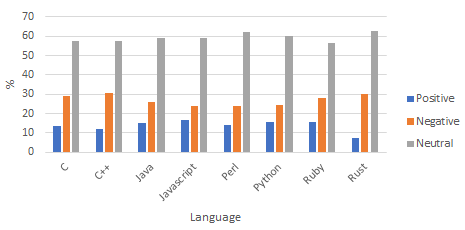
\includegraphics[width=0.49\textwidth]{figures/summNeutralQ.png}}
\caption{Distribution of sentiments in questions.}
\label{fig}
\end{figure}

\begin{figure}[htbp]
\centerline{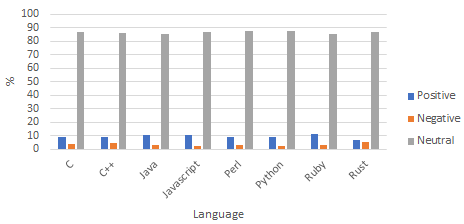
\includegraphics[width=0.49\textwidth]{figures/summNeutralA.png}}
\caption{Distribution of sentiments in answers.}
\label{fig}
\end{figure}

\begin{figure}[htbp]
\centerline{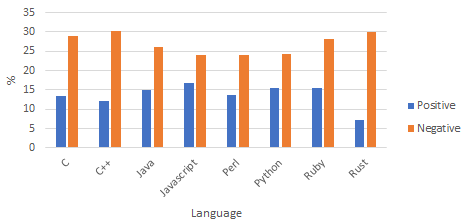
\includegraphics[width=0.49\textwidth]{figures/summQ.png}}
\caption{Distribution of positive/negative sentiments in questions.}
\label{fig}
\end{figure}

\begin{figure}[htbp]
\centerline{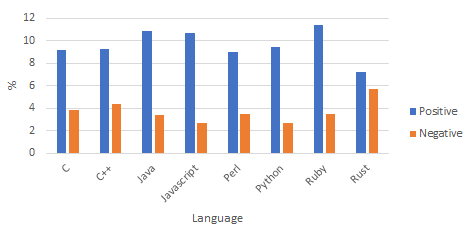
\includegraphics[width=0.49\textwidth]{figures/summA.png}}
\caption{Distribution of positive/negative sentiments in answers.}
\label{fig}
\end{figure}

\subsection{RQ2: Trends over time}
Discussion for this goes here

\begin{figure}[htbp]
\centerline{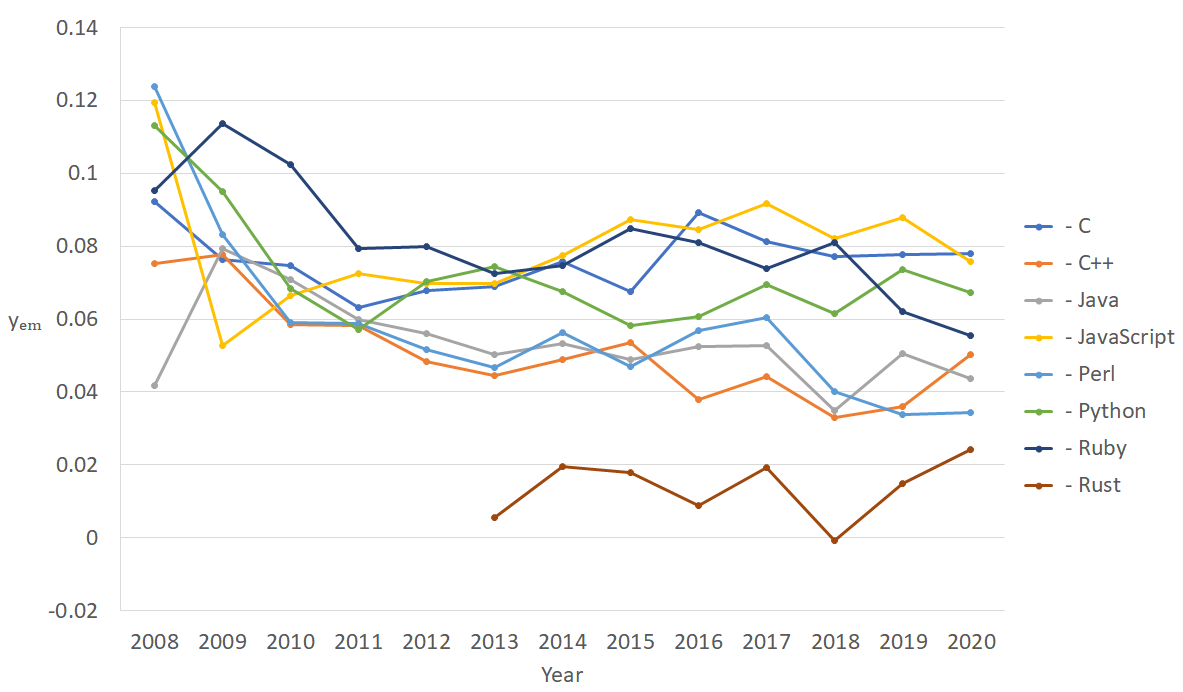
\includegraphics[width=0.49\textwidth]{figures/time_answers_em.png}}
\caption{Answer Sentiments over time.}
\label{fig}
\end{figure}

\begin{figure}[htbp]
\centerline{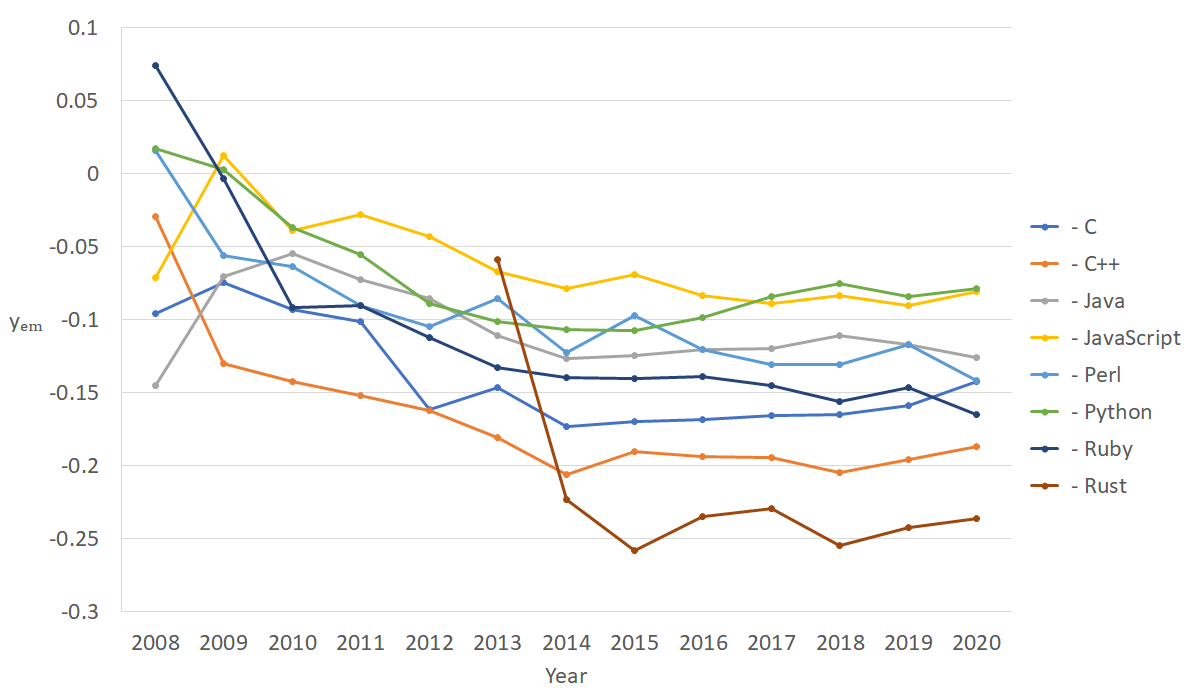
\includegraphics[width=0.49\textwidth]{figures/time_questions_em.png}}
\caption{Question Sentiments over time.}
\label{fig}
\end{figure}

\subsection{RQ3: Interpreted vs Compiled}
Discussion for this goes here

\begin{figure}[htbp]
\centerline{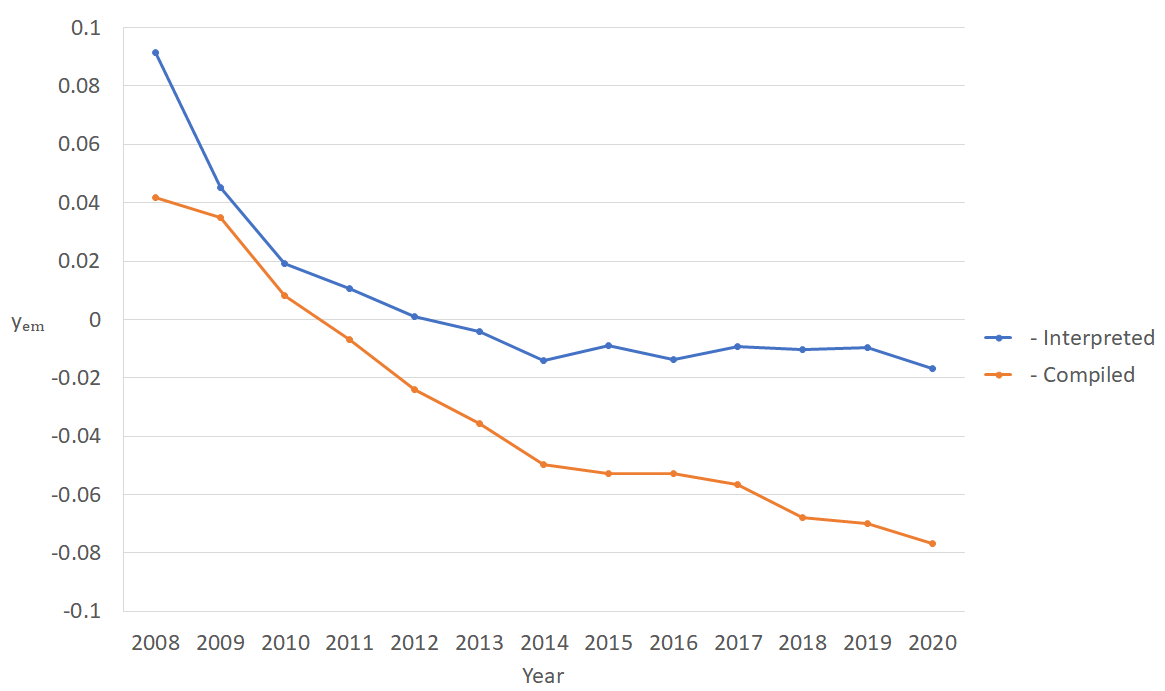
\includegraphics[width=0.49\textwidth]{figures/time_interpreted_compiled.png}}
\caption{Interpreted vs Compiled languages over time.}
\label{fig}
\end{figure}

\subsection{RQ4: Python vs Java}
Discussion for this goes here

\begin{figure}[htbp]
\centerline{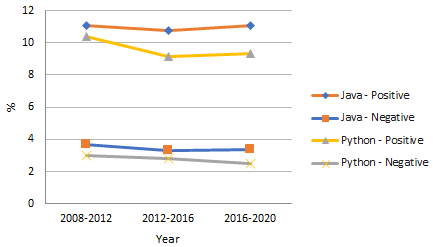
\includegraphics[width=0.49\textwidth]{figures/Java-python-answers.png}}
\caption{Python vs Java answers over the 3 time periods}
\label{fig}
\end{figure}

\begin{figure}[htbp]
\centerline{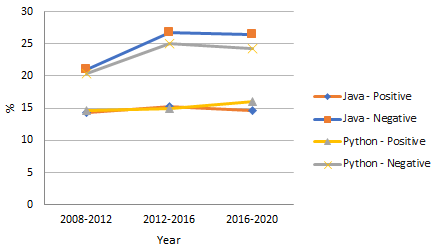
\includegraphics[width=0.49\textwidth]{figures/Java-python-questions.png}}
\caption{Python vs Java questions over the 3 time periods}
\label{fig}
\end{figure}

\begin{figure}[htbp]
\centerline{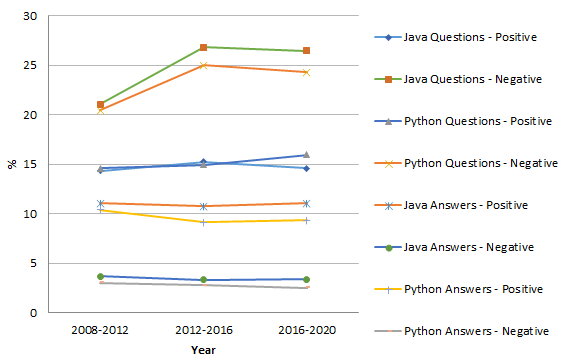
\includegraphics[width=0.49\textwidth]{figures/Java-python-combined.png}}
\caption{Python vs Java questions/answers over the 3 time periods}
\label{fig}
\end{figure}

\subsection{RQ5: Rust is anomalous}
Talking points go here

\begin{figure*}[tbp]
\centering
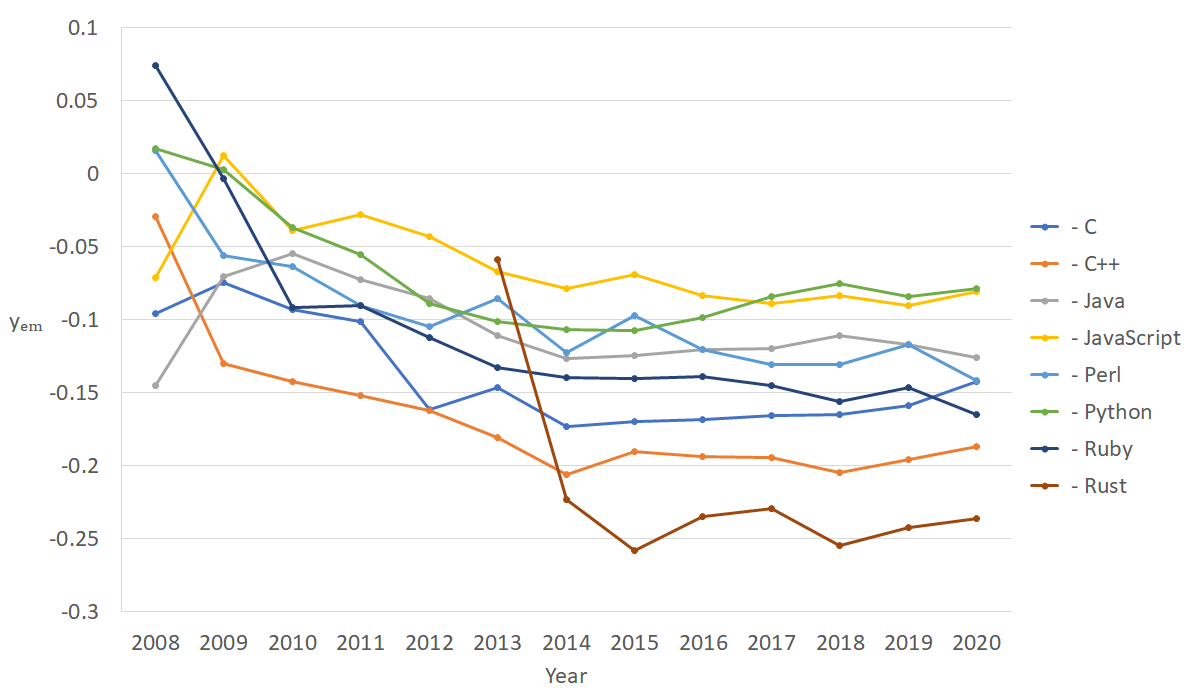
\includegraphics[width=\textwidth]{figures/time_questions_em.png}
\caption{Question Sentiments over time}
\label{fig}
\end{figure*}

\begin{figure*}[tbp]
\centering
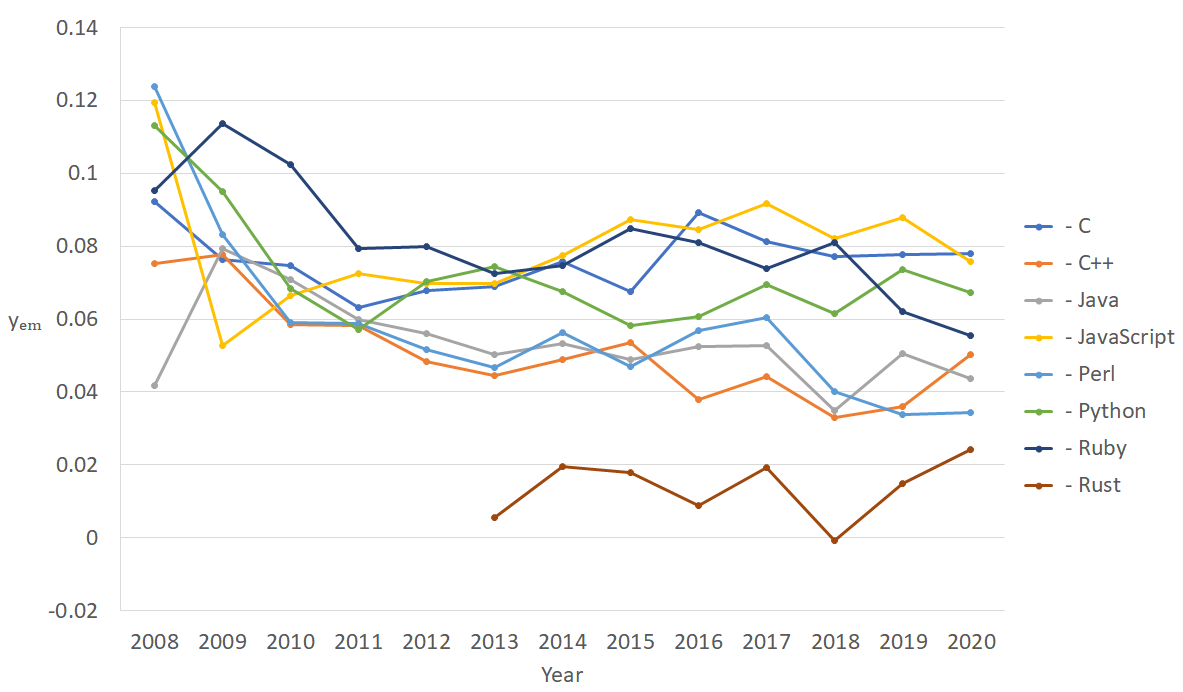
\includegraphics[width=\textwidth]{figures/time_answers_em.png}
\caption{Answer Sentiments Over Time}
\label{fig}
\end{figure*}



\section{Threats to validity}
Stuff that might have introduced errors or how different approach might lead to different conclusions

\section{Conclusion/Future Work}
Summary of results and contributions, and ideas for improvements and future work.\\

\begin{thebibliography}{00}
\bibitem{b1} E. Guzman and B. Bruegge, “Towards emotional awareness in software development teams,” Proceedings of the 2013 9th Joint Meeting on Foundations of Software Engineering - ESEC/FSE 2013, 2013. 

\bibitem{b2} M. D. Choudhury and S. Counts, “Understanding affect in the workplace via social media,” Proceedings of the 2013 conference on Computer supported cooperative work - CSCW '13, 2013. 

\bibitem{b3} F. Calefato, F. Lanubile, M. C. Marasciulo, and N. Novielli, “Mining Successful Answers in Stack Overflow,” 2015 IEEE/ACM 12th Working Conference on Mining Software Repositories, 2015. 

\bibitem{b4} F. Calefato, F. Lanubile, F. Maiorano, and N. Novielli, “Sentiment Polarity Detection for Software Development,” Empirical Software Engineering, vol. 23, no. 3, pp. 1352–1382, 2017. 

\bibitem{b5} F. Calefato, F. Lanubile, and N. Novielli, “How to ask for technical help? Evidence-based guidelines for writing questions on Stack Overflow,” Information and Software Technology, vol. 94, pp. 186–207, 2018. 

\bibitem{b6} “The NEW new ‘Be Nice’ Policy (‘Code of Conduct’) - Updated with your feedback,” Meta Stack Exchange, 2014. [Online]. Available: https://meta.stackexchange.com/questions/240839/the-new-new-be-nice-policy-code-of-conduct-updated-with-your-feedback. [Accessed: 06-Dec-2020]. 

\bibitem{b7} C. A. Thompson, “A Brief Introduction to Natural Language Processing for Non-linguists,” Learning Language in Logic Lecture Notes in Computer Science, pp. 36–48, 2000. 

\bibitem{b8} P. M. Nadkarni, L. Ohno-Machado, and W. W. Chapman, “Natural language processing: an introduction,” Journal of the American Medical Informatics Association, vol. 18, no. 5, pp. 544–551, 2011.

\bibitem{b9} W. G. Cochran, Sampling techniques. New York: John Wiley \& Sons, 1977. 

\bibitem{b10} B. Pang and L. Lee, “Opinion Mining and Sentiment Analysis,” Foundations and Trends® in Information Retrieval, vol. 2, no. 1–2, pp. 1–135, 2008. 

\bibitem{b11} L. Ling and S. Larsén, “Sentiment Analysis on Stack Overflow with Respect to Document Type and Programming Language,” 2018. 

\bibitem{b12} G. D. Israel, “Determining Sample Size,” 1992. 

\bibitem{b13} F. N. Ribeiro, M. Araújo, P. Gonçalves, M. A. Gonçalves, and F. Benevenuto, “SentiBench - a benchmark comparison of state-of-the-practice sentiment analysis methods,” EPJ Data Science, vol. 5, no. 1, 2016. 

\bibitem{b14} H. Tang, S. Tan, and X. Cheng, “A survey on sentiment detection of reviews,” Expert Systems with Applications, vol. 36, no. 7, pp. 10760–10773, 2009. 

\bibitem{b15} A. Esuli and F. Sebastiani, “SentiWordNet: A High-Coverage Lexical Resource for Opinion Mining,” 2007. 

\bibitem{b16} M. Thelwall, K. Buckley, G. Paltoglou, D. Cai, and A. Kappas, “Sentiment strength detection in short informal text,” Journal of the American Society for Information Science and Technology, vol. 61, no. 12, pp. 2544–2558, 2010. 

\bibitem{b17} R. Socher, A. Perelygin, J. Y. Wu, J. Chuang, C. D. Manning, A. Y. Ng, and C. Potts, “Recursive Deep Models for Semantic Compositionality Over a Sentiment Treebank,” Proceedings of the 2013 Conference on Empirical Methods in Natural Language Processing, pp. 1631–1642, Oct. 2013. 

\bibitem{b18} F. Calefato, F. Lanubile, F. Maiorano, and N. Novielli, “Sentiment Polarity Detection for Software Development,” Empirical Software Engineering, vol. 23, no. 3, pp. 1352–1382, 2017. 

\bibitem{b19} T. Ahmed, A. Bosu, A. Iqbal, and S. Rahimi, “SentiCR: A customized sentiment analysis tool for code review interactions,” 2017 32nd IEEE/ACM International Conference on Automated Software Engineering (ASE), 2017. 

\bibitem{b20} M. R. Islam and M. F. Zibran, “Leveraging Automated Sentiment Analysis in Software Engineering,” 2017 IEEE/ACM 14th International Conference on Mining Software Repositories (MSR), 2017.

\bibitem{b21} N. Novielli, D. Girardi, and F. Lanubile, “A benchmark study on sentiment analysis for software engineering research,” Proceedings of the 15th International Conference on Mining Software Repositories, 2018. 

\bibitem{b22} E. Biswas, M. E. Karabulut, L. Pollock, and K. Vijay-Shanker, “Achieving Reliable Sentiment Analysis in the Software Engineering Domain using BERT,” 2020 IEEE International Conference on Software Maintenance and Evolution (ICSME), 2020.

\bibitem{b23} M. Ortu, G. Destefanis, B. Adams, A. Murgia, M. Marchesi, and R. Tonelli, “The JIRA Repository Dataset,” Proceedings of the 11th International Conference on Predictive Models and Data Analytics in Software Engineering - PROMISE '15, 2015.

\bibitem{b24}  N. V. Chawla, K. W. Bowyer, L. O. Hall, and W. P. Kegelmeyer, “SMOTE: Synthetic Minority Over-sampling Technique,” Journal of Artificial Intelligence Research, vol. 16, pp. 321–357, 2002. 

\bibitem{b25} N. Novielli, F. Calefato, and F. Lanubile, “A gold standard for emotion annotation in stack overflow,” Proceedings of the 15th International Conference on Mining Software Repositories, 2018. 

\bibitem{b26} N. Novielli, F. Calefato, F. Lanubile, and A. Serebrenik, “Assessment of SE-specific Sentiment Analysis Tools: An Extended Replication Study,” Oct. 2020.

\bibitem{b27} J. Devlin, M.-W. Chang, K. Lee, and K. Toutanova, “BERT: Pre-training of Deep Bidirectional Transformers for Language Understanding,” May 2019. 

\bibitem{b28} “Browse Queries,” Stack Exchange Data Explorer. [Online]. Available: https://data.stackexchange.com/stackoverflow. [Accessed: 07-Dec-2020]. 

\bibitem{b29} “Stack Overflow Developer Survey 2020,” Stack Overflow, Feb-2020. [Online]. Available: https://insights.stackoverflow.com/survey/2020. [Accessed: 06-Dec-2020]. 

\bibitem{b30} P. Chatterjee, M. Kong, and L. Pollock, “Finding help with programming errors: An exploratory study of novice software engineers’ focus in stack overflow posts,” Journal of Systems and Software, vol. 159, p. 110454, 2020. 

\bibitem{b31} N. Novielli, F. Calefato, D. Dongiovanni, D. Girardi, and F. Lanubile, “Can We Use SE-specific Sentiment Analysis Tools in a Cross-Platform Setting?,” Proceedings of the 17th International Conference on Mining Software Repositories, 2020. 

\bibitem{b32} “Everything There Is to Know about Sentiment Analysis,” MonkeyLearn. [Online]. Available: https://monkeylearn.com/sentiment-analysis/. [Accessed: 06-Dec-2020]. 

\bibitem{b33} N. Novielli, F. Calefato, and F. Lanubile, “Towards discovering the role of emotions in stack overflow,” Proceedings of the 6th International Workshop on Social Software Engineering - SSE 2014, 2014. 

\bibitem{b34} N. Novielli, F. Calefato, and F. Lanubile, “The challenges of sentiment detection in the social programmer ecosystem,” Proceedings of the 7th International Workshop on Social Software Engineering - SSE 2015, 2015. 

\bibitem{b35} M. R. Islam and M. F. Zibran, “A comparison of software engineering domain specific sentiment analysis tools,” 2018 IEEE 25th International Conference on Software Analysis, Evolution and Reengineering (SANER), 2018. 

\bibitem{b36} N. Imtiaz, J. Middleton, P. Girouard, and E. Murphy-Hill, “Sentiment and politeness analysis tools on developer discussions are unreliable, but so are people,” Proceedings of the 3rd International Workshop on Emotion Awareness in Software Engineering, 2018. 

\end{thebibliography}
\vspace{12pt}
\color{red}
NOTE: Sections 3 onwards are still Work in Progress.









 

 
 


 








\end{document}
